% 第3章第6节：指派（指派问题与模型变形；可行标号与紧边证书；匈牙利算法；算法分析、结果检验与问题比较）。

\section{指派}
\label{sec:graph-assignment}

上一节只关心能配上多少对。现在每个对象都必须完成配对，而不同配对的成本不同：把$N$项工作分给$N$名工人，每人做一项，工人$i$做工作$j$的耗时为$c_{i,j}$，要使总耗时最少。可行解仍是二部图中的匹配，而且必须是完美匹配；新增的是边上的成本，以及证明一个解已经最省的手段。

本节先写出指派问题及几种常见变形。随后给行与列配置标号，用它们给出任何完整指派成本的下界，并说明只用“紧边”完成的指派恰好达到这个下界。匈牙利算法同时维护可行标号与由紧边组成的匹配：匹配用上一节的交替路径扩大，扩大不了时调整标号以产生新的紧边。最后分析开销，说明怎样检验结果，并比较最大匹配、指派与最小费用流三种问题。

\subsection{指派问题}
\label{sec:graph-opt-assign-problem}

把工人看成左侧的行，工作看成右侧的列。行$i$与列$j$之间允许配对时，配对成本$c_{i,j}$是有限实数；不允许的配对没有边。

\begin{definition}[指派问题]
\label{def:graph-opt-assignment}
设有$N$行、$N$列，允许的行列对组成边集$E$，每条边$(i,j)\in E$有有限实成本$c_{i,j}$。\term{指派问题}（assignment problem）要求选出一个完美匹配，即给每行指定一个不同的列，并且只用允许边，使总成本$\sum_i c_{i,\sigma(i)}$最小，其中$\sigma(i)$是分给行$i$的列。
\end{definition}

全部行列对都允许时，$\sigma$可以是任意置换，用$0$-$1$变量$x_{i,j}$表示就是每行每列恰选一个元素。行数少于列数的矩形情形，可以补充若干虚拟行，它们到每一列的成本都是零：补成方阵后，虚拟行只占用原来没有被真实行使用的列，总成本不变，删去虚拟行的配对就得到原问题的解。

实际问题中还要分清三种设定。第一种是本节主线，每个对象都必须配对。第二种允许不配对，但未配对要付惩罚。这时不能只把“恰选一次”放宽成“至多选一次”：成本都非负时，什么都不选的空匹配就成了最优解。正确的做法是把惩罚写进模型，例如给每个左侧对象$i$配一个专属虚拟列，配给它的成本是$i$的惩罚$\rho_i$；给每个右侧对象$j$配一个专属虚拟行，成本是$j$的惩罚$\eta_j$；真实对象与非专属虚拟对象之间禁止配对，虚拟行与虚拟列之间成本为零。这样补成的方阵中，完整指派的成本恰为真实配对成本加上未配对对象的惩罚。第三种设定是某些配对被禁止，这由边集$E$表达。若某一行没有任何允许边，或者一组行能使用的列总数少于行数，就不存在完美匹配，必须报告不可行，而不是给出一个使用禁止配对的“解”。

指派也可以写成上一节与第~\ref{sec:graph-min-cost-flow}节的模型：令每行供给$1$、每列需求$1$，每条允许边是容量为$1$、单位费用为$c_{i,j}$的弧，则整数可行流与完美匹配一一对应，费用就是指派成本。由树流的整数性，网络单纯形法在这个网络上给出的最优流是整数流，所以可以直接用它求解。尽管如此，本节仍利用二部配对的结构设计专门算法：模型之间可以转换，并不意味着必须采用同一个求解过程。

\subsection{可行标号与最优性条件}
\label{sec:graph-opt-assign-labels}

最小费用流用节点势给出最优性证书。在指派问题中，同样的思想可以写得更直接：给每行、每列各配一个数，用它们给出任意完整指派成本的一个下界。以下设问题已补成$N$阶方阵，每行每列恰配一次。

给每行$i$配实数$u_i$，每列$j$配实数$v_j$。若对每条允许边都有
\begin{equation}
  u_i+v_j\leq c_{i,j},
  \label{eq:graph-opt-feasible-labels}
\end{equation}
就称$(\bm u,\bm v)$为\term{可行标号}（feasible labeling）。对任意完整指派$\sigma$，把它用到的$N$条边的不等式相加，每行恰出现一次、每列也恰出现一次，于是
\[
  \sum_{i=1}^Nc_{i,\sigma(i)}\geq\sum_{i=1}^N\bigl(u_i+v_{\sigma(i)}\bigr)=\sum_{i=1}^Nu_i+\sum_{j=1}^Nv_j.
\]
右边与$\sigma$无关，是全部完整指派成本的共同下界。这个论证只依赖“每行每列恰计一次”，不需要一般的线性规划对偶理论。在上一小节的流模型中把$\pi_i=u_i$、$\pi_j=-v_j$看成节点势，$c_{i,j}-u_i-v_j$就是行到列弧的约化费用，可行标号对应全部约化费用非负。

使式~\eqref{eq:graph-opt-feasible-labels}取等号的边称为\term{紧边}（tight edge），$c_{i,j}-u_i-v_j$称为边的剩余量。

\begin{theorem}[紧边指派的最优性]
\label{thm:graph-opt-tight-assignment}
设$(\bm u,\bm v)$是可行标号。若完整指派$\sigma$只使用紧边，则它的成本等于$\sum_iu_i+\sum_jv_j$，因而是最优指派。
\end{theorem}

\begin{proof}
$\sigma$用到的每条边都取等号，上面的求和不等式也取等号，所以$\sigma$的成本等于下界。任何完整指派的成本都不低于这个下界，所以$\sigma$最优。
\end{proof}

于是求解指派问题的任务变成两件同时进行的事：保持标号可行，同时在紧边中寻找完美匹配。可行标号本身只提供下界；在找到全由紧边组成的完整指派之前，不能宣称已经得到最优解。

\subsection{匈牙利算法}
\label{sec:graph-opt-hungarian}

\term{匈牙利算法}（Hungarian algorithm）从一组容易得到的可行标号和空匹配出发，只在紧边上扩大匹配；当紧边不够用时，修改标号以制造新的紧边，同时保证已有的紧边匹配不被破坏。

\paragraph{初始可行标号}
先检查每行至少有一条允许边，否则直接报告不可行。取每行的最小允许成本作为行标号$u_i=\min_{j:\,(i,j)\in E}c_{i,j}$，列标号全取零。每条允许边满足$u_i+0\leq c_{i,j}$，标号可行，并且每行至少有一条紧边。

\paragraph{交替树的生长}
从一个自由行出发，在紧边上用上一节的交替搜索建立\term{交替树}（alternating tree）：从行出发只走紧的非匹配边到列；若到达的列已经匹配，就沿匹配边回到它的配对行，继续扩展；若到达自由列，从树根到该列的路径就是一条由紧边组成的增广路径，沿它翻转，匹配增加一条边，然后从下一个自由行重新建树。树中每个列都与树中某一行匹配，每个非根行都是从它的配对列走进来的，所以若记树中的行集为$S$、列集为$T$，则$|S|=|T|+1$，多出的一行就是自由的树根。

\paragraph{标号调整}
如果交替树不能再扩展，说明从$S$出发的紧边都通向$T$。这时在$S$到树外列的允许边中求最小剩余量
\begin{equation}
  \delta=\min\bigl\{c_{i,j}-u_i-v_j:\ i\in S,\ j\notin T,\ (i,j)\in E\bigr\},
  \label{eq:graph-opt-hungarian-delta}
\end{equation}
并令$S$中各行的标号加$\delta$、$T$中各列的标号减$\delta$。由于树外的这些边都不紧，$\delta>0$。逐类检查这一调整的效果。两端分别在$S$与$T$中的边，$u_i+v_j$不变，树中的紧边和匹配边都保持紧，交替树完整保留。行在$S$、列不在$T$的边，剩余量减少$\delta$，由$\delta$的取法仍然非负，取到最小值的边变成紧边，于是交替树至少可以多扩展一步。行不在$S$、列在$T$的边，剩余量增加$\delta$；其余的边不变。匹配边要么两端都在树中，要么两端都在树外，所以全部保持紧。调整后标号仍然可行，而标号下界$\sum u_i+\sum v_j$增加了$|S|\delta-|T|\delta=\delta$。

若式~\eqref{eq:graph-opt-hungarian-delta}中的候选集合为空，$S$中各行的允许列全部落在$T$中，$|S|$行只能使用$|T|=|S|-1$个列，不可能各配一个不同的列，于是报告不可行，而不是虚构一个有限的步长。

\begin{algorithm}[匈牙利算法]
\label{alg:graph-opt-hungarian}
输入：$N$阶方阵形式的指派问题（允许边集与成本）。输出：最优完整指派与可行标号，或“不可行”的结论。状态：行列标号、紧边匹配、交替树的行集$S$与列集$T$、各列的前驱、未入树列的最小剩余量。
\begin{enumerate}
  \item 若某行没有允许边，报告不可行；否则取$u_i$为第$i$行最小允许成本、$v_j=0$，匹配为空。
  \item 若所有行都已匹配，转第5步；否则取一个自由行作为交替树的根，令$S$只含它、$T=\varnothing$。
  \item 从$S$中的行沿紧的非匹配边扩展到列，已匹配的列沿匹配边把它的配对行加入$S$。若到达自由列，沿前驱翻转增广路径，回到第2步。
  \item 若树不能再扩展：候选集合为空则报告不可行；否则按式~\eqref{eq:graph-opt-hungarian-delta}求$\delta$，$S$中行标号加$\delta$、$T$中列标号减$\delta$，回到第3步。
  \item 输出匹配与标号；若曾补充虚拟行或虚拟列，按原始模型删去或解释相应配对。
\end{enumerate}
\end{algorithm}

在整个过程中，有三条性质始终保持：标号可行，匹配只用紧边，交替树中的边都是紧边。增广只改变匹配，不改变标号；调标号只改变标号，不破坏已有的紧边匹配与交替树。全部行都匹配时，匹配是一个只由紧边组成的完整指派，由定理~\ref{thm:graph-opt-tight-assignment}，它是最优的。所以这个算法不只是一串对成本矩阵的减法操作，每一步都维护着一份可以随时核对的下界。

\paragraph{算例}
成本矩阵为
\[
  \bm C=\begin{bmatrix}1&2\\1&100\end{bmatrix}.
\]
逐行贪心时，第一行先取最便宜的第$1$列，成本$1$，第二行只剩第$2$列，成本$100$，合计$101$。另一种指派是第一行配第$2$列、第二行配第$1$列，成本为$2+1=3$。贪心的问题在于两行都最偏爱第$1$列，而第二行失去它的代价远大于第一行。

匈牙利算法取初始标号$u=(1,1)$、$v=(0,0)$，紧边为$(1,1)$与$(2,1)$。第一行沿紧边到达自由的第$1$列，直接配对。第二行出发建树：沿紧边到第$1$列，第$1$列已配给第一行，把第一行加入树；第一行的紧边只有到第$1$列的那一条，树无法扩展，如图~\ref{fig:graph-opt-hungarian}(a)。此时$S=\{1,2\}$，$T=\{1\}$，树外列只有第$2$列，剩余量分别为$c_{1,2}-u_1-v_2=1$与$c_{2,2}-u_2-v_2=99$，所以$\delta=1$。

调整后$u=(2,2)$、$v=(-1,0)$。边$(1,1)$与$(2,1)$的剩余量仍为零，边$(1,2)$的剩余量变为$2-2-0=0$，成为新的紧边，边$(2,2)$的剩余量为$98$。交替树从第一行扩展到自由的第$2$列，得到增广路径：第二行—第$1$列—第一行—第$2$列，如图~\ref{fig:graph-opt-hungarian}(b)。翻转后第二行配第$1$列，第一行配第$2$列，成本为$2+1=3$；标号下界为$2+2+(-1)+0=3$，两者相等，图~\ref{fig:graph-opt-hungarian}(c)的指派最优。

\begin{figure}[!htb]
  \centering
  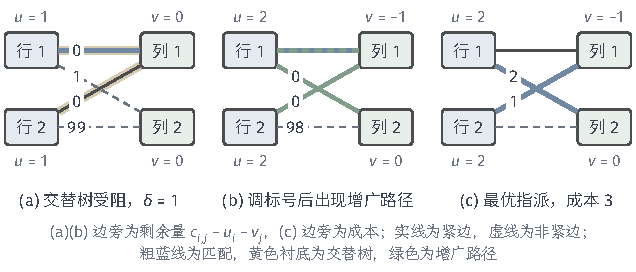
\includegraphics[width=107.714mm]{figures/01-basic-mathematics/04-graphs/tikz/c3-assign-hungarian/figure.pdf}
  \caption{匈牙利算法在成本矩阵$\left[\begin{smallmatrix}1&2\\1&100\end{smallmatrix}\right]$上的运行。行、列旁为当前标号。(a)匹配为行$1$配列$1$，从自由的行$2$出发的交替树（黄色衬底）只到达列$1$与行$1$，树外边的最小剩余量为$\delta=1$。(b)行标号加$1$、树中列标号减$1$后，行$1$到列$2$变紧，出现增广路径（绿色）。(c)翻转得到的指派成本为$3$，等于标号之和。}
  \label{fig:graph-opt-hungarian}
\end{figure}

\paragraph{停止与还原}
全部行都匹配后停止。若为矩形问题补过零成本虚拟行，删去它们的配对即得原问题的解；若按惩罚模型补过专属虚拟行列，配给专属虚拟对象的真实对象就是未配对的对象，总成本中相应的项就是它的惩罚。禁止的配对从未作为允许边出现，所以不会出现在结果中。

\subsection{算法分析与结果检验}
\label{sec:graph-opt-assign-analysis}

\paragraph{计算开销}
朴素地实现，每次调标号都要扫描$S$中全部行到树外全部列的剩余量。更好的做法是为每个未入树的列$j$维护最小剩余量$\min_{i\in S}(c_{i,j}-u_i-v_j)$及取到最小值的行，作为这一列的前驱。有一行加入$S$时，用它到各列的剩余量更新这些最小值，花$O(N)$；求$\delta$只需在这些最小值中再取最小，花$O(N)$；调标号后，未入树列的最小剩余量统一减去$\delta$，也是$O(N)$。为一个自由行建树直到增广，至多有$N$行加入$S$、至多调标号$N$次，所以一次增广为$O(N^2)$；至多增广$N$次，稠密$N$阶方阵上的总运算量为$O(N^3)$次实数运算。存储上，原始成本表占$N^2$个数，这是输入本身；算法额外的工作数组为$O(N)$。

\paragraph{结果检验}
先检查原始问题的可行性：每行恰配一个列，所用的列互不相同，全部配对都是允许边；再按原始成本重算总成本。然后检查证书：对全部允许边验证$u_i+v_j\leq c_{i,j}$，对所选的边验证取等号，并核对总成本等于$\sum_iu_i+\sum_jv_j$。原始可行解的成本等于标号下界，才构成最优性证书。浮点实现中，“紧”与“可行”都只能在容差内判断，应说明所用容差；近似相等不能无条件替代精确证书。

\paragraph{三种问题的比较}
最大匹配、指派与最小费用流可以互相转写，但目标与约束不同。最大匹配只求配对数量，边上没有成本；指派要求每个对象都完成配对，在这一条件下比较成本；最小费用流允许一般的容量、上下界与供需，指派只是全部容量为一、每行供给一、每列需求一的特例。图~\ref{fig:graph-opt-problem-relations}汇总了这些关系。专门算法保留了各自的结构：增广匹配只需记录配对伙伴，匈牙利算法的标号与交替树都利用了二部结构，网络单纯形法则适用于一般网络。算法名称不是不改模型就能互换的工具，换用另一种算法之前，须先把问题按它的输入要求重新写出。

\begin{figure}[!htb]
  \centering
  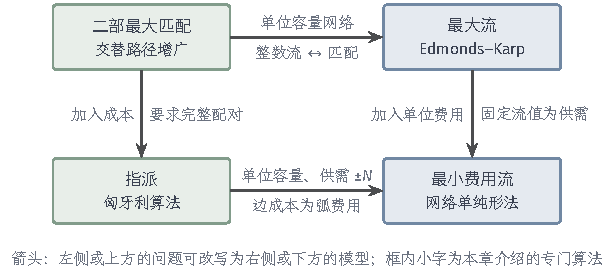
\includegraphics[width=103.914mm]{figures/01-basic-mathematics/04-graphs/tikz/c3-problem-relations/figure.pdf}
  \caption{本章四种流与配对问题之间的模型关系。箭头表示起点的问题可以写成终点的模型：二部最大匹配是单位容量的最大流，加入成本并要求完整配对就成为指派；最大流固定流值并加入单位费用就成为最小费用流，指派是单位容量的最小费用流。框内小字是本章为各问题介绍的专门算法。}
  \label{fig:graph-opt-problem-relations}
\end{figure}
